\chapter{Técnicas básicas e ferramentas utilizadas}

\textbf{Introduzir o capítulo quando tudo já estiver escrito.}
%Neste capítulo, serão descritas técnicas básicas de Aprendizado de Máquina e Processamento de Linguagem Natural, importantes para a compreensão dos capítulos seguintes desta monografia. Na seção \textbf{Classificadores}, serão discutidos os funcionamentos dos classificadores Naïve Bayes e \emph{Support Vector Machines} (SVMs), comuns em métodos de Mineração de Perspectiva baseados em frequências de palavras. Na seção \textbf{Modelos Gráficos}, serão discutidas a notação e hipóteses deste tipo de modelo, os \textbf{Modelos Generativos}, uma de suas subcategorias bastante explorada nesta monografia, e dois modelos generativos que, a partir da interpretação de documentos como uma mistura de tópicos, geram agrupamentos de palavras que facilitam a compreensão segmentada do conteúdo de um corpus. Estes modelos são o \emph{Latent Dirichlet Allocation} (LDA) e o \emph{Labeled-Latent Dirichlet Allocation} (L-LDA), utilizados em experimentos conduzidos ao longo de todo o projeto.

%\textbf{serão discutidos os modelos de tópicos \emph{Latent Dirichlet Allocation} (\textbf{LDA}) e \emph{Labeled Latent Dirichlet Allocation} (\textbf{L-LDA}). O segundo, que consiste em uma pequena modificação do primeiro, é utilizado em parte dos experimentos conduzidos neste projeto.}


\section{Modelos Gráficos}

%\begin{figure}[t]
%  \centering % este comando é usado para centralizar a Figura
%  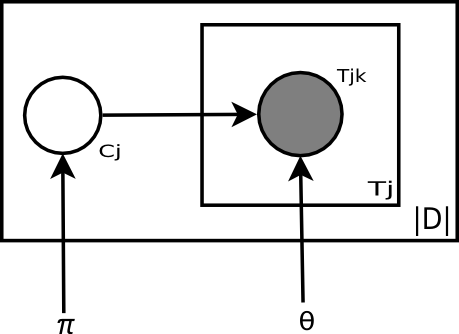
\includegraphics[width=5cm, height=4cm]{graphical-naive.png}\\
%  \caption{Modelo gráfico do Naïve Bayes.}
%  \label{fig:graphical-naive}
%\end{figure}


\begin{figure}[t]
  \centering % este comando é usado para centralizar a Figura
  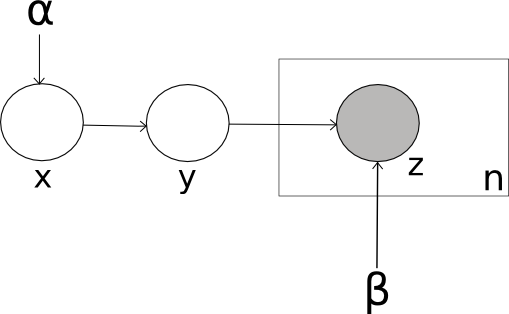
\includegraphics[width=5cm, height=3.4cm]{exemplo-modelo-grafico.png}\\
  \caption{Exemplo de modelo gráfico.}
  \label{exemplo:grafico}
\end{figure}



%\begin{figure}[t]
%  \centering % este comando é usado para centralizar a Figura
%  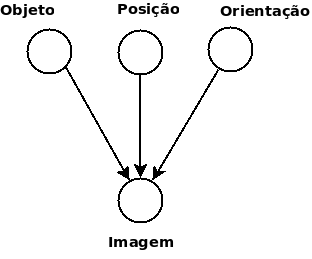
\includegraphics[width=5cm, height=4cm]{generative-bishop.png}\\
%  \caption{Modelo gráfico que representa o processo pelo qual objetos são gerados probabilisticamente. A distribuição de probabilidade para a imagem depende da identidade do objeto, de sua orientação e de sua posição \cite{bishop}.}
%  \label{fig:generative-bishop}
%\end{figure}

Modelos gráficos consistem na representação, através de um grafo, das relações entre um conjunto finito de variáveis aleatórias, provendo uma maneira simples de se representar distribuições de probabilidade \cite{bishop}. Cada vértice do grafo corresponde a uma variável aleatória (ou a um conjunto de variáveis aleatórias) ou a um parâmetro do modelo, e cada aresta reflete a relação entre dois vértices. Modelos gráficos são categorizados como dirigidos ou não-dirigidos. Por questões de escopo, apenas modelos dirigidos (também conhecidos como Redes Bayesianas) serão discutidos nesta seção.

Em um modelo gráfico dirigido, tem-se um grafo direcionado acíclico que representa a distribuição de probabilidade conjunta\footnote{Nesta monografia, os termos "distribuição de probabilidade conjunta" e "distribuição conjunta" serão utilizados de forma intercambiável.} para suas variáveis aleatórias. Cada aresta corresponde a uma distribuição de probabilidade condicional, incidindo no vértice cuja distribuição de probabilidade está condicionada ao valor do vértice de onde ela parte. Quando mais de uma variável tem distribuição de probabilidade condicionada aos mesmos vértices, é possível sintetizar a notação representando todas elas com um único vértice. Neste caso, o vértice fica dentro de um retângulo rotulado com o número de variáveis que ele representa. 

Por fim, vértices representados com círculos brancos correspondem a variáveis latentes - ou seja, cujos valores não são observáveis diretamente no conjunto de dados ao qual o modelo é aplicado; círculos cinzas, por sua vez, correspondem a variáveis observáveis, cujos valores estão explícitos no conjunto de dados. Variáveis latentes permitem que distribuições de probabilidade muito complexas, envolvendo variáveis observáveis, sejam construídas a partir de distribuições condicionais mais simples \cite{bishop}. A Figura \ref{exemplo:grafico} corresponde a um modelo gráfico com a seguinte distribuição conjunta

\begin{equation}
\label{eq:fiction}
\ensuremath{P(x | \alpha)P(y | x)\prod_{i=1}^{n}P(z_i | y, \beta)} 
\end{equation}

\ensuremath{\alpha} e \ensuremath{\beta} são parâmetros de distribuições de probabilidade, \ensuremath{x} e \ensuremath{y} são variáveis latentes e \ensuremath{z_1, ..., z_n}, sintetizadas na Figura \ref{exemplo:grafico} através do vértice \ensuremath{z}, são variáveis observáveis.


%A \textbf{Joint Distribution} do classificador Naïve Bayes, que corresponde ao produto de todas as distribuições de probabilidade do modelo, pode ser escrita como 

% rótulo indica o número de variáveis. % esta represehaja, no modelo, um certo número de variáveis aleatórias que dependem 

 

%\textbf{********** Pensar num jeito de explicar a notação sem falar de Naïve Bayes. Falar de variáveis latentes e observáveis. *****************}

%\textbf{                                                                                The
%primary role of the latent variables is to allow a complicated distribution over the
%observed variables to be represented in terms of a model constructed from simpler
%(typically exponential family) conditional distributions.}

%\subsubsection{Modelos Generativos} 

Uma categoria de modelos gráficos explorada neste projeto são os \textbf{modelos generativos}. Eles associam distribuições de probabilidade a todas as variáveis aleatórias envolvidas, permitindo a geração - i.e. simulação - de seus valores. Modelos generativos são úteis para expressar os processos pelos quais dados observáveis são obtidos. Em um modelo deste tipo, os valores das variáveis aleatórias podem ser obtidos através de técnicas de amostragem aplicadas à distribuição de probabilidade conjunta. Além do Naïve Bayes, discutido na seção \ref{subsection:naive}, os modelos gráficos generativos \emph{Latent Dirichlet Allocation} (LDA) e \emph{Labeled Latent Dirichlet Allocation} (L-LDA) foram empregados em experimentos ao longo de todo o projeto. Uma discussão sobre eles pode ser encontrada na seção \ref{subsection:LDA}. %, como no seguinte exemplo: dado um conjunto de imagens de objetos, variáveis latentes podem ser utilizadas para representar suas posições e orientações; em seguida, para identificar o objeto contido em uma imagem particular observada, deve-se obter a distribuição de probabilidade a posteriori para objetos, o que envolve integrar sobre todas as posições e orientações possíveis \cite{bishop}. A Figura \textbf{2.2} indica as distribuições de probabilidade envolvendo variáveis aleatórias para posição, orientação, imagem e objeto.  %, como será discutido, no caso particular do modelo Naïve Bayes, na seção \ref{subsection:naive}.

%, como a amostragem de Gibbs apresentada na seção 2.1.1. É um mecanismo diferente do empregado em SVMs, por exemplo, em que variáveis observáveis não são associadas a nenhuma distribuição de probabilidade e as categorias são estimadas diretamente, condicionadas a seus valores. SVMs estão apresentados com mais detalhes na seção 2.1.2. \textbf{Acho q a monografia n precisa falar de modelos discriminativos.}

 %  modelo de tópicos L-LDA, que consiste em uma alteração simples no modelo LDA. Estes últimos, discutidos na seção \ref{subsection:LDA}, %, bem como o classificador Naïve Bayes.

\subsection{Naïve Bayes}
\label{subsection:naive}

O Naïve Bayes é um modelo gráfico generativo utilizado para a geração de documentos em \emph{datasets} particionados em classes. Ele é estudado em sete dos treze trabalhos revisados para essa monografia, onde funciona como base para a classificação de documentos de acordo com suas perspectivas\footnote{Assume-se, nesses estudos, que cada classe corresponde a uma perspectiva e cada documento se associa a apenas uma classe.}. Trata-se, portanto, de um modelo bastante explorado na área de Mineração de Perspectiva, que normalmente conduz a bons resultados na tarefa de classificação. Por questões de estrutura, nesta seção serão apresentadas apenas as hipóteses, parâmetros e distribuições de probabilidade associadas ao modelo. Na seção \ref{subsection:bayes}, a sua utilização como classificador será discutida em detalhes.

%Ele é utilizado como base para classificação de documentos estudado por sete dos treze muito utilizado nos trabalhos revisados n

Dado um corpus \ensuremath{D}, particionado no conjunto de classes \ensuremath{C} e com um vocabulário \ensuremath{V}\footnote{Em alguns casos, pode-se assumir que \ensuremath{V} é composto de outras características dos documentos, em vez de suas palavras. Elas podem ser, por exemplo, sequências de duas palavras presentes em \ensuremath{D} (bigramas).}, o Naïve Bayes assume que os \ensuremath{|D|} documentos são gerados a partir de distribuições de probabilidade específicas de cada classe \ensuremath{c \in C}, definidas através de um conjunto de parâmetros \ensuremath{\phi = \{\pi, \theta_{1}, ..., \theta_{|C|}\}}. Além disso, o modelo também assume que as palavras em qualquer documento ocorrem independentemente umas das outras - ou seja, elas são \textbf{condicionalmente independentes} \cite{nigam}. %Além disso, esse modelo também desconsidera a ordem em que as palavras aparecem nos documentos \cite{nigam}. 


No Naïve Bayes, um documento \ensuremath{d_i} é gerado a partir da (1) seleção de uma classe \ensuremath{c_j}, de acordo com as distribuições de probabilidade \ensuremath{P(c_j | \phi)}, e (2) a geração do documento em si, com distribuição de probabilidade \ensuremath{P(d_i | c_j ; \phi)} \cite{mccallum-nigam}. Como \ensuremath{d_i} é uma lista de \ensuremath{|d_i|} palavras, \ensuremath{< w_{d_{i,1}}, ..., w_{d_{i,|d_i|}} >}, gerá-lo  corresponde a amostrar cada uma delas. Assumindo-se que elas ocorrem no documento independentemente umas das outras, a probabilidade de se gerar  \ensuremath{d_i}, dado \ensuremath{\phi}, pode ser reescrita como \cite{nigam}  

\begin{equation}
\label{gerando-di}
\ensuremath{P(d_i | \phi) = \sum_{j = 1}^{|C|}\bigg(P(c_j | \phi)\prod_{k = 1}^{|d_i|}P(w_{d_{i,k}} | c_j ; \theta)\bigg)}
\end{equation}

Existe um parâmetro \ensuremath{\pi} responsável por \emph{regular} a probabilidade de que uma determinada classe seja selecionada na geração de um documento \ensuremath{d_i}. A probabilidade de se obter uma palavra \ensuremath{w_t \in V}, na \ensuremath{k}-ésima posição de \ensuremath{d_i} dada uma classe \ensuremath{c_j}, também depende da \ensuremath{t}-ésima posição de um parâmetro \ensuremath{\theta_j} - \ensuremath{\theta_j^{(t)}}. O conjunto de parâmetros \ensuremath{\phi}, portanto, define distribuições de probabilidade para palavras e classes do corpus \ensuremath{D} \cite{nigam}. Essas relações estão ilustradas na Figura \ref{naive:joint}, que corresponde à distribuição de probabilidade conjunta do modelo Naïve Bayes.

\begin{figure}[h]
 \centering % este comando é usado para centralizar a Figura
 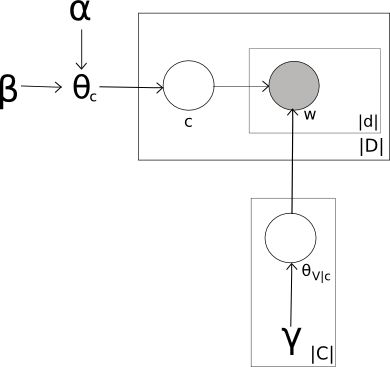
\includegraphics[width=6cm, height=5.6cm]{naive-joint.png}\\
 \caption{Modelo gráfico Naïve Bayes.}
 \label{naive:joint}
\end{figure}

Quando se deseja gerar um documento, sem o compromisso de se aproximar as distribuições para as classes e palavras o máximo possível daquelas presentes no corpus, pode-se definir os valores de \ensuremath{\phi} através da simples amostragem dos parâmetros \ensuremath{\phi' = \{\alpha_{1}, ..., \alpha_{|C|}, \gamma_1, ..., \gamma_{|C|}\}}. Os elementos de \ensuremath{\phi'} recebem o nome de \textbf{hiperparâmetros}, por \emph{regularem} distribuições de probabilidade para os parâmetros do modelo. Seus valores devem ser escolhidos antes de se começar o processo de geração de \ensuremath{d_i}. Nesse projeto e em todos os outros estudados para essa monografia, há apenas duas classes em \ensuremath{D}, de modo que a distribuição Beta pode ser utilizada na amostragem de \ensuremath{\pi}

\begin{equation}
\label{theta_c}
  \ensuremath{\pi \sim Beta(\alpha, \beta)}  
\end{equation}

Dada uma classe \ensuremath{c_j}, a sua distribuição de palavras é \emph{regulada} por um parâmetro \ensuremath{\theta_j}, amostrado de acordo com

\begin{equation}
\label{theta_j}
  \ensuremath{\theta_j \sim Dirichlet(\gamma_j)}
\end{equation}

Com valores para \ensuremath{\phi}, a classe de \ensuremath{d_i} pode ser amostrada de acordo com uma distribuição \ensuremath{Binomial(|C| - 1, \pi)}; cada uma de suas palavras \ensuremath{w_{d_{i,k}}}, por sua vez, corresponde à \ensuremath{k}-ésima posição da amostra obtida através da distribuição \ensuremath{Multinomial(V, |d_i|, \theta_j)}.

Em um contexto de classificação, como será discutido na seção \ref{subsection:bayes}, os valores de \ensuremath{\phi} devem maximizar a probabilidade de se obter os documentos de um corpus \ensuremath{D}. Como não é possível obter, com uma quantidade finita de dados, os valores mais prováveis de  \ensuremath{\phi} para a geração de \ensuremath{D} \cite{nigam}, eles são estimados. Isso conduz a aproximações de \ensuremath{P(c_j | \phi)} e \ensuremath{P(d_i | c_j ; d_i)}.





% e não se sabe de antemão quantos pertencem a cada classe, é possível amostrar todos os valores de \ensuremath{\phi} .... 

%assume-se que todos os \ensuremath{|C|} parâmetros \ensuremath{\theta_{c_j}} possuem o mesmo valor inicial. Essa estratégia é interessante em um contexto de classificação, conforme será discutido na seção \ref{subsection:bayes}. Esse valor é amostrado de acordo com uma distribuição de probabilidade \textbf{a priori}, definida pelos parâmetros \ensuremath{\alpha} e \ensuremath{\beta}. Os valores iniciais dos \ensuremath{|C|} parâmetros \ensuremath{\theta_{ V | c_j}}, por sua vez, são amostrados de acordo com distribuição de probabilidade definida pelos parâmetros \ensuremath{\gamma_j, j \in \{1, ..., |C|\}}. Os parâmetros \ensuremath{\alpha, \beta} e \ensuremath{\gamma_j, j \in \{1, ..., |C|\}}, recebem o nome de \textbf{hiperparâmetros},  Na seção \ref{subsection:bayes}, a reamostragem desses parâmetros também é discutida em detalhes. Por ora, é suficiente informar que, inicialmente, um documento \ensuremath{d_i} pode ser gerado de acordo com as seguintes distribuições de probabilidade:


 %Cada classe corresponde a uma variável latente e todas as palavras são 
% Também em um contexto de classificação, amostram-se valores iniciais para os parâmetros  \ensuremath{\theta_{c_j 


 %de acordo com distribuições de probabilidade \textbf{a priori}, definidas pelos parâmetros \ensuremath{\alpha, \beta} e  A reamostrage



%Com isso, torna-se 
%a escolha de qualquer classe equiprovável, Como nesse contexto há documentos cujas classes não são conhecidas de antemão, essa estratégia torna a escolha de qualquer classe equiprovável.

%                         θwt|cj : wt ∈
%V, cj ∈ C ; θcj : cj ∈ C



%                                         written θcj , which indicate the probabilities
%of selecting the different mixture components.


 %Nesse modelo, cada classe \ensuremath{c \in C} é uma variável latente. Mais especificamente, portanto, tem-se que o parâmetro de \ensuremath{\ensuremath{\pi \in \theta} é responsável %; cada palavra \ensuremath{w \in V}, uma variável observável.
%O conjunto de parâmetros \ensuremath{\theta}, base para as distribuições é composto, portanto,  é Portanto os parametros de cada classe definem uma distribuição multinomial sobre palavras, ie, a coleção de probabilidades de palavras, cada uma escrita como theta_{w_t|c_j) tal q esse bicho é "três traços" P(w_t|c_j; theta) onde t = {1, ..., |V|} e o somatorio dessas P's, variando t, dá 1. Como se assume q para todas as classes o tamanho do documento é distribuído de forma idêntica, ele n precisa ser parametrizado pra classificação. Os únicos parametros do modelo são as prob. das classes, theta_c_j, que indicam as probabilidades de se obter classes diferentes. Os modelos do parametro, portanto, definindo um conjunto de multinomials e class prob's é theta = {theta_wt|cj : wt \in V, c_j \in C; theta_cj : c_j \in C}.



%\prod_{i = 1}^{n} p(v_{di} |  c)}

%di é uma lista ordenada de palavras <w_{di,1}, w_{di,2}, ...>. w_{d_{i,k}] é a palavra w_t na posição k de d_i, onde w_t pertence a V = <w_1, ..., w_|V|>. Dê um exemplo! Se esse paragrafo fosse documento 3, w_7,3 seria uma. O tamanho do documento, |d_i|, é escolhido antes e independent. da classe. Daí, a partir da classe selecionada, se gera |d_i| palavras. A geração de cada palavra tb independe do tamanho do documento.

%P(d_i| c_j; theta) = P(|d_i) * prod. (k = 1 a |d_i|) de P(w_{d_{i,k}}|cj; theta, w_{d_{i,q}}, q < k) => a probabilidade de se obter uma palavra é condicionada a todas as palavras obtidas antes.

%Maaaaas, no Naïve Bayes, as palavras são geradas independentemente de contexto - ou seja, independentemente de outras palavras no mesmo documento dada a classe. A prob. de uma palavra tb independe de sua posição no documento. Isso quer dizer q fica

%P(d_i|c_j; theta) = P(|d_i)prod de k = 1 a d_i de P(w_d_i,k | c_j, theta)


% permite que se gere um documento , pertencente a uma classe \ensuremath{c_j \in C}, de acordo com a distribuição de probabilidade definida pelo seu conjunto de parâmetros, denominado \ensuremath{\theta}. O doc



%Informalmente, para se gerar um documento \ensuremath{d_i}, seleciona-se uma classe \ensuremath{c_j} e, em seguida, baseando-se nessa informação e no conjunto \ensuremath{\theta}, seleciona-se cada uma de suas \ensuremath{|d_i|} palavras, contidas em \ensuremath{V}. A probabilidade de se gerar um \ensuremath{d_i} qualquer, portanto, é dada por 

%\begin{equation}
%\label{gerando-di}
%\ensuremath{c \sim Binomial(|C| - 1, \pi)}
%\end{equation}
%O documento \ensuremath{d_i} é gerado através da seleção de uma classe \ensuremath{c_j}, cuja distribuição de probabilidade é \ensuremath{P(c_j | \theta)}, e, em seguida,  

% Primeiramente, seleciona-se uma classe \ensuremath{c_j} de acordo com a distribuição de probabilidade  e, em seguida, gera-se \ensuremath{d_i}

%                                             A document, di , is created by first select-


% Informalmente, seleciona-se uma classe \ensuremath{c_j} e em seguida, 

%Primeiramente, seleciona-se uma das \ensuremath{|C|} classes \ensuremath{c \in C}, de acordo com % das palavras nos documentos. Para o Naïve Bayes, \emph{tênis de mesa} e \emph{de mesa tênis}


%Sem perda de generalidade, assume-se que \ensuremath{c} é uma variável aleatória que pode assumir \ensuremath{m} valores naturais distintos, variando de 0 a \ensuremath{m - 1}. Cada valor corresponde a uma classe diferente, sendo escolhido de acordo com  







%   Formally, every document is generated according to a probability distribution
%defined by the parameters for the mixture model, denoted θ.


% é um modelo generativo, ele permite que se simule a criação de um documento \ensuremath{d}, pertencente a uma classe \ensuremath{c}, através da amostragem de suas variáveis aleatórias. 


%Implicit in this model are the assumptions that (1)
%documents are generated from class-specific probability distributions, and (2) words
%occur in documents independently of each other given the class.

% assume a independência condicional das características \ensuremath{F_1, ..., F_k} presentes em um conjunto de documentos \ensuremath{D}. Se \ensuremath{D} é composto de documentos de texto, estas características normalmente correspondem a todas as suas palavras distintas. Isto equivale a assumir, portanto, que a presença de uma palavra em um documento qualquer não é informativa sobre a presença de nenhuma outra. 

%A finalidade básica do Naïve Bayes é estimar a probabilidade de um documento \ensuremath{d} pertencer a uma certa classe \ensuremath{c}. Para isto, \ensuremath{d} é representado de forma simplificada, através de um vetor \ensuremath{v_d} em que cada posição corresponde a uma de suas \ensuremath{n} palavras. Com esta representação, a probabilidade de \ensuremath{d} pertencer a uma classe \ensuremath{c} pode ser calculada via Teorema de Bayes como

%variáveis aleatórias, em que \ensuremath{d_i denota a relevância de F_i para d}. \textbf{MEXER NESSA EXPLICAÇÃO!} \ensuremath{d_i} pode ser a frequência de \ensuremath{F_i} em \ensuremath{d}, ou indicar sua presença com o valor 1 e sua ausência com o valor 0, por exemplo. 

%\begin{equation}
%\label{eq1:naive}
%\ensuremath{P(c | v_{d1}, ..., v_{dn}) = \frac{p(c) \times p(v_{d1}, ..., v_{dn} | c)}{p(F_1, ..., F_k)} }
%\end{equation}

%Como o Naïve Bayes assume que as palavras dos documentos são condicionalmente independentes, a equação \ref{eq1:naive} pode ser reescrita como 

%\begin{equation}
%\label{eq2:naive}
%\ensuremath{P(c | v_{d1}, ..., v_{dn}) = \frac{p(c) \times p(v_{d1} |  c)p(v_{d2} | c)...p(v_{dn - 1} | c)p(v_{dn} | c)}{p(F_1, ..., F_k)} = \frac{p(c) \times \prod_{i = 1}^{n} p(v_{di} |  c)}{p(F_1, ..., F_k)}}
%\end{equation}

%Na \textbf{seção XXX}, a equação \ref{eq2:naive} será retomada para a discussão sobre como construir um classificador a partir do modelo Naïve Bayes.



% Após uma classe ter sido fixada de acordo com \ref{eq3:label-naive}, seleciona-se uma palavra para cada posição \ensuremath{j} do vetor \ensuremath{v_d}, de acordo com uma distribuição de probabilidade sobre \ensuremath{F_1, ..., F_k}

%\begin{equation}
%\label{eq5:multi-naive}
%\ensuremath{v_{dj} \sim Multinomial(F_1, ..., F_k, \theta_c)}
%\end{equation}

%A distribuição utilizada depende do valor de \ensuremath{c} amostrado anteriormente, de modo que há \ensuremath{m} parâmetros \ensuremath{\theta_c}. Cada \ensuremath{\theta_c} é escolhido antes do processo de geração dos documentos, de acordo com

%\begin{equation}
%\label{eq6:theta-naive}
%\ensuremath{\theta_c \sim Dirichlet(\gamma_c)}
%\end{equation}

%\ensuremath{\gamma_c}, assim como \ensuremath{\alpha} e \ensuremath{\beta}, é um hiperparâmetro.

%A distribuição conjunta para este modelo generativo é dada por

%\begin{equation}
%\label{eq7:joint-naive}
%\ensuremath{P(\pi | \alpha, \beta)\prod_{i = 0}^{m - 1}P(\theta_{c = i} | \gamma_{c=i})\prod_{j = 1}^{|D|}P(c_j | \pi)P(v_d^{(j)} | \theta_{c_j}, c_j)}
%\prod_{i = 0}^{m - 1}P(c = i | \pi)P(\theta_{c = i} | \gamma_{c = i})P(v_d^{(j)} | \theta_{ c = i})} 
%\end{equation}



%em que \ensuremath{c_j} é a classe selecionada para o \ensuremath{j}-ésimo documento de \ensuremath{D} e \ensuremath{v_d^{(j)}} é seu vetor de palavras. A Figura \ref{naive:joint} representa esta distribuição conjunta de forma gráfica, com vértices para variáveis aleatórias e relações de probabilidade condicional evidenciadas pelas arestas.


% Caso haja \ensuremath{m} classes, tem-se que a classe de \ensuremath{d
 % Assume-se que há uma variável aleatória para cada \ensuremath{f \in F}, cujos valores denotam a relevância de cada uma delas para um \ensuremath{d} fixado. %Estas variáveis podem assumir valores discretos, como a contagem de quantas vezes elas ocorreram em \ensuremath{d}os valores 1 e 0, caso façam parte ou não do documento \ensuremath{d} e 0 em caso contrário, ou contí relevância pode ser medida binariamente - \ensuremath{1 se f é uma das palavras de d, 0 em caso contrário} -  %, e a presença ou ausência de uma delas em um documento qualquer é independente da presença ou ausência de qualquer outra. 

% parte da ideia de que as informações presentes em um documentoe, são independentes entre si. No caso de um documento de texto, assume-se que 




%associa uma classe a cada documento de um corpus. 

% No caso do classificador Naïve Bayes - modelo gráfico que, por conveniência, é discutido mais detalhadamente na seção \ref{subsection:bayes} -, tem-se variáveis aleatórias que representam a classe de cada documento e, para todos os documentos, variáveis aleatórias para cada um de seus termos distintos. Este modelo contém dois parâmetros, \ensuremath{\pi} e \ensuremath{\theta}, que ajustam as distribuições de probabilidade das variáveis aleatórias. 


%Este tipo de classificador parte da ideia de que as informações presentes em um documento, utilizadas na determinação de sua classe, são independentes entre si. No caso de um documento de texto, assume-se que a presença ou ausência de um termo - uma palavra ou uma sequência de palavras - é independente da presença ou ausência de qualquer outro. Definida esta hipótese, a probabilidade de que um documento \emph{d} seja de uma classe \emph{c} é tal que

%\begin{equation}
%label{eq1}
%\ensuremath{P(c|d) \propto P(c)\prod_{k=1}^{t_d}P(t_k|c)}  
%\end{equation} 

%onde \ensuremath{P(t_k|c)} é a probabilidade condicional do termo \ensuremath{t_k}  ocorrer em um documento da classe \ensuremath{c},  \ensuremath{P(c)} é a probabilidade a priori de um documento qualquer pertencer à classe \ensuremath{c} e \ensuremath{t_d} é o número de termos em \emph{d} \cite{stanford-IRbook}.

%As probabilidades envolvidas na relação \ref{eq1} contêm integrais díficeis ou mesmo impossíveis de se calcular analiticamente. Para calcular \ensuremath{P(c|d)}, portanto, utiliza-se aproximações obtidas através de técnicas de amostragem. Uma destas técnicas, comum na literatura de Aprendizado de Máquina e empregada neste projeto, é a amostragem de Gibbs. Em uma iteração da amostragem, a técnica condiciona as probabilidades calculadas para um documento \ensuremath{k} às classificações obtidas para os \ensuremath{k - 1} documentos anteriores \cite{resnik-gibbs}. A técnica está descrita, de forma básica, no algoritmo \textbf{X (o algorithm2e.sty tá dando pau)}.
                             % The basic idea in Gibbs sampling is that, rather than probabilistically picking
%the next state all at once, you make a separate probabilistic choice for each of the k dimensions, where each
%choice depends on the other k − 1 dimensions.


%A hipótese de independência entre os termos, razão pela qual o Naïve Bayes tem este nome\footnote{Naïve é uma palavra de origem francesa que significa "ingênua"}, simplifica bastante a estrutura da informação contida nos documentos. Ainda assim, o classificador costuma apresentar boas performances em categorização de textos, sendo utilizado, por exemplo, como base metodológica para alguns filtros de \emph{spam} \cite{paul}. Para melhorar o desempenho do Naïve Bayes, é comum fixar um conjunto de documentos previamente classificados de forma correta e utilizar a informação sobre suas classes na determinação das classes de outros documentos. Ao conjunto de documentos previamente classificados, dá-se o nome de \textbf{conjunto de treinamento}; ao conjunto de documentos a serem classificados, \textbf{conjunto de teste}.

%Todos os experimentos com Naïve Bayes conduzidos neste projeto utilizam a implementação disponível no repositório \emph{online} de Aline Bessa \cite{alibezz-nb}. O número de iterações para a Amostragem de Gibbs foi fixado em 500. %Através do uso de Amostragem de Gibbs, a cada iteração se obtém uma aproximação melhor O número de amostras coletadas envolvendo cada classe foi fixado em 500. 



%A Figura 2.1, correspondente ao classificador Naïve Bayes, contém toda a notação necessária para as discussões sobre modelos gráficos deste projeto. Assume-se que o classificador será aplicado a um conjunto de documentos \ensuremath{D}. A classe de cada documento \ensuremath{j}, \ensuremath{C_j}, é uma variável aleatória com distribuição de probabilidade \ensuremath{P(C_j|\pi)}. A relação entre \ensuremath{C_j} e \ensuremath{\pi}, evidenciada em \ensuremath{P(C_j|\pi)}, é representada na Figura 2.1 pela aresta que sai de \ensuremath{\pi} e incide em \ensuremath{C_j}. \ensuremath{C_j} está no interior de um retângulo rotulado com \ensuremath{|D|}, o que significa que há \ensuremath{|D|} variáveis deste tipo, uma para cada documento. %, com \ensuremath{j} variando de 1 a \ensuremath{N}. 

%Cada documento \ensuremath{j}, por sua vez, contém um conjunto de \ensuremath{T_j} termos distintos. A probabilidade associada a cada termo \ensuremath{T_{jk}}, \ensuremath{k} variando de 1 a \ensuremath{T_j}, é condicionada ao valor da variável \ensuremath{C_j}. Desse modo, e considerando o parâmetro \ensuremath{\theta}, tem-se, por documento, \ensuremath{T_j} distribuições de probabilidade do tipo \ensuremath{P(T_{jk}|C_j, \theta)}. Uma vez mais, o rótulo do retângulo mais interno indica o número de variáveis, sintetizadas por um único círculo, que estabelecem o mesmo tipo de relação com \ensuremath{\theta} e \ensuremath{C_j}. %no modelo. 

%Por fim, as variáveis representadas por círculos brancos são latentes - ou seja, seus valores não são observáveis diretamente no conjunto de dados ao qual o modelo é aplicado. As variáveis em cinza, por sua vez, correspondem a dados diretamente observáveis; neste caso, às palavras distintas de cada documento. A \textbf{Joint Distribution} do classificador Naïve Bayes, que corresponde ao produto de todas as distribuições de probabilidade do modelo, pode ser escrita como 

%\begin{equation}
%\label{generative:eq1}
%\ensuremath{\prod_{j=1}^{|D|} \bigg\{P(C_j|\pi)\bigg[\prod_{k=1}^{T_j}P(T_{jk}|C_j)\bigg]\bigg\}}  
%\end{equation} 

%Adequando-se a notação, observa-se que a relação \ref{eq1}, apresentada na seção 2.1.1, pode ser facilmente obtida via a \textbf{Joint Distribution} \ref{generative:eq1}.

%\subsubsection{Modelos Generativos} 

%Uma categoria de modelos gráficos explorada neste projeto são os Modelos Generativos. Modelos deste tipo associam distribuições de probabilidade a todas as variáveis aleatórias envolvidas, permitindo a geração - i.e. simulação - de seus valores. Modelos generativos são úteis para expressar os processos pelos quais dados observáveis são obtidos, como no seguinte exemplo: dado um conjunto de imagens de objetos, variáveis latentes podem ser utilizadas para representar suas posições e orientações; em seguida, para identificar o objeto contido em uma imagem particular observada, é preciso obter a distribuição de probabilidade a posteriori para objetos, o que envolve integrar sobre todas as posições e orientações possíveis \cite{bishop}. A Figura 2.2 indica as distribuições de probabilidade envolvendo variáveis aleatórias para posição, orientação, imagem e objeto.

%Com um modelo generativo, os valores das variáveis podem ser obtidos através de técnicas de amostragem aplicadas à \textbf{Joint Distribution}, como a amostragem de Gibbs apresentada na seção 2.1.1. É um mecanismo diferente do empregado em SVMs, por exemplo, em que variáveis observáveis não são associadas a nenhuma distribuição de probabilidade e as categorias são estimadas diretamente, condicionadas a seus valores. SVMs estão apresentados com mais detalhes na seção 2.1.2. \textbf{Acho q a monografia n precisa falar de modelos discriminativos.}

%Dois modelos generativos são bastante explorados nos capítulos seguintes desta monografia: o classificador Naïve Bayes e o modelo de tópicos L-LDA, que consiste em uma alteração simples no modelo LDA. Estes últimos, discutidos na seção \ref{subsection:LDA}, foram empregados em experimentos e estudos de caso ao longo de todo o projeto. %, bem como o classificador Naïve Bayes.


% são mapeados em categorias baseando-se nesta informação condicionando 


%os valores das variáveis latentes são associados a distribuições de probabilidade que as condicionam a variáveis observ condicionados a variáveis observadas explicitamente.

%por exemplo, em que o valor de uma variável aleatória


%Discriminative models differ from generative models in that they do not allow one to generate samples from the joint distribution of x and y.
% Quando uma técnica de amostragem adequada é aplicada ao modelo, a fim de obter valores para suas variáveis, tem-se a simulação de dados cuja distribuição de probabilidade aproxima-se daquela dos dados 

%\textbf{Figura do bayes}
%\textbf{Figura bishop com legenda}    

%=> Falar de modelos generativos e fazer link com o resto da seção.
% A independência condicional \pi é um hiperparâmetro do modelo, e a caixa mais externa, rotulada com um \ensuremath{N}, indica que \ensuremath{j} varia de 1 a \a relação entre \ensuremath{\pi} e as variáveis   

\subsection{LDA}
\label{subsection:LDA}


O modelo LDA parte da ideia de que um documento pode tratar de múltiplos tópicos, refletidos nas palavras que o compõem \cite{pnas}. Assim como no modelo Naïve Bayes, palavras podem ser geradas de acordo com distribuições multinomiais específicas. A diferença é que, no LDA, cada palavra é gerada a partir de uma mistura de tópicos; no Naïve Bayes, elas são geradas a partir de um só tópico (classe) \cite{gibbs-lingpipe}.

O LDA associa as palavras dos documentos a tópicos diferentes, com maior ou menor probabilidade, criando agrupamentos que se relacionam semanticamente. Os tópicos em um LDA são variáveis latentes, cujos significados requerem uma interpretação posterior ao processamento. Esta interpretação baseia-se nas relações semânticas entre as palavras que se associaram mais fortemente a cada um deles. %, algo relativamente subjetivo. %ser bastante levando  

Para ilustrar como as palavras evidenciam o significado de um tópico, um experimento envolvendo receitas culinárias extraídas do \emph{site} \textbf{allrecipes.com} foi executado. Apenas os ingredientes de cada receita foram considerados. Na Tabela 2.1, constam as cinco palavras mais fortemente associadas a quatro tópicos, de acordo com o LDA. % - ou seja, as cinco palavras para as quais as probabilidades obtidas com a equação \ref{eq2} foram mais altas. %que obtiveram mais alta probabilidade de acordo com \ref{eq2}.

\begin{table}[t]
\centering
\label{LDA:1}
\begin{tabular}{| l | p{7cm} | }
\hline
\textbf{Tópico} & \textbf{Palavras} \\ \hline
\textbf{Tópico 1} & beef, cheese, tomato, sauce, pepper \\ \hline
\textbf{Tópico 2} & chicken, breast, pastum, broth, tomato \\ \hline
\textbf{Tópico 3} & flour, sugar, butter, powder, egg  \\ \hline
\textbf{Tópico 4} & cream, cheese, butter, milk, cake \\ \hline
\end{tabular}
\caption{As cinco palavras mais fortemente associadas a quatro tópicos gerados por um LDA.}
\end{table}

Considerando que todas as receitas pertencem à culinária tradicional dos Estados Unidos, as palavras listadas na Tabela 2.1, e a forma como se associam em torno de cada tópico, são indicativos do bom funcionamento do LDA. O primeiro tópico pode ser interpretado como \textbf{ingredientes para          \emph{cheeseburger}}; o segundo, ao associar \emph{chicken}, \emph{pastum} e \emph{broth}, remete a receitas de sopas e caldos comuns em climas frios, podendo ser interpretado como \textbf{ingredientes para sopa}; o terceiro pode ser interpretado como \textbf{ingredientes para bolo}; o quarto, ao associar \emph{cream}, \emph{cheese} e \emph{cake}, pode ser interpretado como \textbf{ingredientes para \emph{cheesecake}}. É importante frisar que estas interpretações, apesar de subjetivas, indicam perspectivas culinárias distintas e coerentes internamente. Seria diferente de encontrar, por exemplo, um tópico fortemente associado às palavras \emph{sugar}, \emph{pepper} e \emph{potato}, dificilmente encontradas em uma mesma receita típica dos Estados Unidos.


%- ou seja, não são identificados antes ou durante o processamento -cujos significados requerem  só podem ser interpretados após o processamento do modelo, observando-se  

% que, após o processamento, sintetizam um significado associado ao


%atribuir um significado a cada um deles apenas observando as relações entre as palavras associadas com mais destaque. Para o LDA, os tópicos não são, portanto, pré-identificados antes do processamento, requerendo uma interpretação posterior e subjetiva de seus significados. %Neste sentido, o modelo é útil para identificar padrões contidos em documentos de texto.  

O modelo LDA trata cada documento pertencente a um conjunto de documentos \ensuremath{D} como uma mistura de tópicos, representada por uma distribuição de probabilidade sobre um conjunto de tópicos \ensuremath{T}. Cada tópico, por sua vez, é visto como uma mistura de palavras, representada por uma distribuição sobre todas as palavras distintas de \ensuremath{D}. Para cada documento \ensuremath{d \in D}, é fixada uma distribuição de probabilidade sobre tópicos \ensuremath{\theta_d}, condicionada a um hiperparâmetro \ensuremath{\alpha}

\begin{equation}
\label{lda:topic}
\ensuremath{\theta_d \sim Dirichlet(\alpha)}
\end{equation}

Para cada tópico \ensuremath{t \in T}, é fixada uma distribuição de probabilidade \ensuremath{\phi_t} sobre palavras, condicionada a um hiperparâmatro \ensuremath{\beta}

\begin{equation}
\label{lda:word}
\ensuremath{\phi_t \sim Dirichlet(\beta)}
\end{equation}

Em seguida, para cada uma das \ensuremath{n} palavras de \ensuremath{d}, um tópico \ensuremath{t} é escolhido, de acordo com \ensuremath{\theta_d}

\begin{equation}
\label{lda:topic-chosen}
\ensuremath{t \sim Discrete(\theta_d)}
\end{equation}

e uma palavra \ensuremath{w} é gerada de acordo com \ensuremath{\phi_t}

\begin{equation}
\label{lda:word-chosen}
\ensuremath{w \sim Discrete(\phi_t)}
\end{equation}

A distribuição conjunta do modelo LDA é dada por

\begin{equation}
\label{joint:lda}
\ensuremath{\prod_{i=1}^{|D|} \bigg\{P(\theta_i|\alpha)\bigg[\prod_{j=1}^{|W|}P(t_j|\theta_i)P(w_j|t_j,\beta)\bigg]\bigg\}}  
\end{equation}

\ensuremath{P(w_j|t_j,\beta)} reflete o quanto a palavra \ensuremath{w_j} se relaciona com o tópico \ensuremath{t_j}; \ensuremath{P(t_j|\theta_i)}, por sua vez, funciona como uma medida do quanto o tópico \ensuremath{t_j} é importante no contexto do documento \ensuremath{d_i} \cite{pnas}. Na Figura \ref{fig:lda}, tem-se o modelo gráfico do LDA correspondente à distribuição conjunta \ref{joint:lda}. 

\begin{figure}[t]
  \centering % este comando é usado para centralizar a Figura
  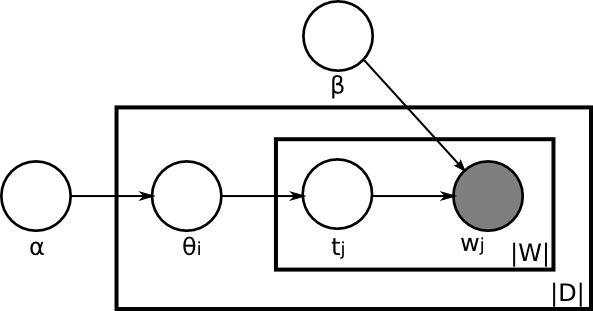
\includegraphics[width=6.5cm, height=3.2cm]{Latent_Dirichlet_allocation.png}\\
  \caption{Modelo gráfico LDA.} %\ref{joint:lda}.}
  \label{fig:lda}
\end{figure}

A implementação do LDA utilizada para estes experimentos está disponível no repositório \emph{online} de Alexandre Passos \cite{top-lda}, e o número de iterações para amostragem de tópicos e palavras foi fixado em 100. 


%O cálculo destas probabilidades também envolve integrais difíceis, ou mesmo impossíveis, de resolver analiticamente, o que implica no uso de técnicas de amostragem e aproximação. A amostragem de Gibbs, descrita superficialmente na seção \ref{subsection:bayes}, é uma alternativa para a geração de valores para variáveis aleatórias contidas no modelo \cite{gibbs-lingpipe}, sendo utilizada nos experimentos com LDA conduzidos neste projeto. 

%Quando um método de classificação é aplicado a um conjunto de documentos, a interpretação do resultado é imediata: cada documento estará associado a uma única classe. No caso do modelo de tópicos LDA, a interpretação do resultado é mais subjetiva. É preciso observar as palavras que se associam com maior probabilidade a cada tópico, buscando algum tipo de semelhança entre elas, para inferir seus significados. 


% o agrupamento de palavras como \emph{beef}, \emph{sauce} e \emph{cheese} em torno de um mesmo tópico indica o bom funcionamento do LDA%As palavras associadas a cada tópico siderando que as receitas pertencem à culinária tradicional dos Estados Unidos. O primeiro tópico pode ser interpretado como \textbf{Receitas com Carne}, pois associa ingredientes comumente consumidos  
%\textbf{Análise}

\subsubsection{L-LDA}

O L-LDA é uma variação do LDA em que se restringe o número de tópicos associados a cada documento. Ou seja, as distribuições fixadas para os tópicos de cada documento não necessariamente são sobre todos os tópicos \ensuremath{t \in T}. Além disso, os tópicos presentes em cada documento são identificados antes da execução do modelo, o que diminui a subjetividade envolvida na interpretação de seus significados após o processamento. 

Um bom exemplo para ilustrar a aplicação deste modelo envolve um \emph{blog}, em que cada \emph{post} é marcado com um conjunto específico de \emph{tags}. Se cada \emph{tag} é interpretada como um tópico, é possível informar ao L-LDA em que \emph{posts} cada uma delas está presente, processar os \emph{posts} com o modelo e saber, após o processamento, quais palavras se associam mais fortemente a cada \emph{tag}. Neste exemplo, existe um mapeamento direto entre os tópicos e as \emph{tags}, conduzindo a uma interpretação mais imediata do significado de cada agrupamento de palavras.

Experimentos com o L-LDA foram desenvolvidos ao longo deste projeto, associando cada tópico, por exemplo, a uma perspectiva a ser minerada. Após a execução do modelo, as palavras mais fortemente associadas a cada perspectiva ilustram como os assuntos discutidos são enfocados por elas. Quanto mais duas perspectivas se distanciam, mais diferentes são as palavras que se associam com destaque a cada uma delas.

O L-LDA foi discutido pela primeira vez em um artigo de Ramage et al. \cite{llda}, aplicado ao problema de atribuição de crédito em páginas do \emph{site del.icio.us}, marcadas com múltiplas \emph{tags}. O artigo parte da hipótese de que, embora um documento possa estar marcado com várias \emph{tags} diferentes, nem sempre elas se aplicam igualmente a todas as palavras nele contidas. A ideia da atribuição de crédito, portanto, consiste em associar cada palavra do documento às \emph{tags} mais apropriadas e vice-versa. 

%Uma aplicação de L-LDA, sugerida neste artigo e bastante empregada neste projeto, envolve, após a associação de palavras a tópicos (neste caso, \emph{tags}), a extração de trechos do documento que as contenham. Isto conduz a uma compreensão melhor de como o conteúdo se associa aos tópicos separadamente. 

A implementação de L-LDA utilizada neste projeto também está disponível no repositório \emph{online} de Alexandre Passos \cite{top-llda}. O número de iterações para amostragem de tópicos e palavras, em todos os experimentos, foi fixado em 100.
% do envolvendo uma ou mais palavras associadas a uma \emph{tag} particular. 
%O resultado de um método de classificação consiste em associar cada documento de um conjunto Diferentemente de métodos de classificação, cujo resultado pode ser interpretado de forma obj

%Assim como discutido na seção \ref{subsection:bayes}, 
% tópicos é fixada multinomial  \ensure\ensuremath{d} se associa a tópicos \ensuremath{t \in T} com probabilidades diferentes, o que é determinado pela escolha de uma distribuição de probabilidade sobre os tópicos. Em seguida, cada tópico é tratado como uma distribuição sobre palavras e cada palavra \ensuremath{w_i} de \ensuremath{d} se associa a eles de acordo com estas distribuições. A probabilidade da \ensuremath{i}-ésima palavra de \ensuremath{d} pode ser calculada como 

%P(wi) = sum P(wi | ti = j) P(ti = j), j de 1 a T. 

%onde ti é uma variável latente - ou seja, cujo valor não é observável, mas sim inferido - referente a um tópico, P(wi | ti = j) é a probabilidade de wi se associar ao tópico j e P(ti = j) é a probabilidade de se obter o tópico j na distribuição fixada para o documento \ensuremath{d} \cite{pnas}.

 %\textbf{Falar das receitas.}
%\textbf{Falar do uso de Gibbs Sampling para inferência}


%\subsection{L-LDA}


\section{Classificadores}

A classificação de documentos de texto de acordo com suas perspectivas é um dos principais objetivos dos trabalhos revisados neste projeto. Grande parte deles utiliza os classificadores Naïve Bayes ou \emph{Support Vector Machines} (SVMs), apresentados respectivamente nas seções \ref{subsection:naive} e \ref{subsection:SVMs}, como parte de suas metodologias. O desempenho destes classificadores é comumente medido através das seguintes métricas: \textbf{taxa de acerto}, \textbf{precisão}, \textbf{rechamada} ou \textbf{métrica F1}.

A taxa de acerto é definida pela razão entre o número de documentos classificados corretamente e todos os documentos avaliados. A precisão, medida para uma classe \ensuremath{c} qualquer, é definida pela razão entre o número de documentos classificados corretamente como \ensuremath{c} e todos os documentos classificados como \ensuremath{c}. A rechamada, medida também para uma classe \ensuremath{c} qualquer, é definida pela razão entre o número de documentos classificados corretamente como \ensuremath{c} e a soma deste valor com o número de documentos classificados erroneamente para todas as demais classes. A métrica F1, também medida para uma classe \ensuremath{c} qualquer, é dada por

\begin{equation}
\ensuremath{2 \times \frac{precisao \times rechamada}{precisao + rechamada}}
\end{equation} 

Estas métricas revelam aspectos diferentes do desempenho de um classificador. Por este motivo, é comum encontrar mais de uma delas sendo utilizada no mesmo contexo. Além de medirem desempenho, elas estabelecem critérios objetivos para a comparação entre métodos de classificação, como pode ser visto nos artigos de Lin et al. sobre o conflito Israel-Palestina \cite{lin-et-al2006} e de Efron sobre orientação cultural \cite{efron}. 

\subsection{Naïve Bayes}
\label{subsection:bayes}

O modelo Naïve Bayes, apresentado na seção \ref{subsection:naive}, pode ser utilizado como base para a construção de um classificador. É dessa forma que ele é empregado nos trabalhos estudados para este projeto. O cenário da classificação abordado nessa monografia envolve um conjunto de documentos \ensuremath{D'}, cujas classes são conhecidas pelo classificador, e um conjunto de documentos \ensuremath{D''}, para o qual isso não vale. O corpus \ensuremath{D} é a união desses dois conjuntos, sendo \ensuremath{D'} utilizado como \textbf{conjunto de treinamento} e \ensuremath{D''}, como \textbf{conjunto de teste}\footnote{O termo \emph{treinamento} é utilizado, em contraposição a \emph{teste}, porque o classificador não precisa inferir as classes dos documentos desse primeiro conjunto. Apesar disso, embora o termo não transpareça, o classificador também pode utilizar informações do conjunto de teste para adaptar melhor suas inferências às características do corpus. Isso é evidenciado nas relações \ref{classe2} e \ref{palavra}.}.


 A classificação em si aplica-se apenas ao conjunto de teste. Cada documento deve ser rotulado com apenas uma classe pertencente ao conjunto \ensuremath{C}, e o vocabulário do corpus, bastante explorado na classificação, corresponde ao conjunto \ensuremath{V}. % enquanto o segundo 

Dado o conjunto de parâmetros \ensuremath{\phi} do modelo Naïve Bayes, \ensuremath{\phi = \{\pi, \theta_1, ..., \theta_{|C|}\}}, tem-se que, pelo Teorema de Bayes, a probabilidade da classe de \ensuremath{d_i \in D''}, \ensuremath{y_i}, ser \ensuremath{c_j} é dada por

\begin{equation}
\label{teorema-bayes}
\ensuremath{P(y_i = c_j | d_i ; \phi) = \frac{P(c_j | \phi)\prod_{k = 1}^{|d_i|}P(w_{d_{i,k}} | c_j; \phi)}{P(d_i | \phi)}}
\end{equation}

O valor que maximiza a função \ref{teorema-bayes} corresponde à classe amostrada para \ensuremath{d_i}. Na prática, como esse é um problema de maximização e a probabilidade \ensuremath{P(d_i | \phi)} independe de qualquer classe, ela pode ser abstraída. Como apresentado na seção \ref{subsection:naive}, os valores dos elementos de \ensuremath{\phi} devem, ns classificação, maximizar a probabilidade de se obter o corpus \ensuremath{D} - ou seja, devem maximizar \ensuremath{P(D | \phi)} \cite{nigam}. Como a obtenção exata desses valores não é possível com um conjunto finito de dados, eles são estimados a partir dos hiperparâmetros de suas distribuições e de informações extraídas do corpus \cite{nigam}. A derivação dessas estimativas não será exposta nessa monografia por questões de escopo, podendo ser conferida no relatório de Bob Carpenter \cite{gibbs-lingpipe}. Elas conduzem às aproximações \ref{classe2} e \ref{palavra}. A probabilidade de se obter a classe \ensuremath{c_j} é aproximada, portanto, através de 

% É trivial observar que os dois termos do numerador dessa função correspondem ao processo generativo do documento \ensuremath{d_i}, apresentado na seção \ref{subsection:naive}: primeiramente, fixa-se uma classe de acordo com  \ensuremath{P(c_j | \phi)}; em seguida, geram-se as \ensuremath{|d_i|} palavras do documento, de acordo com \ensuremath{\prod_{k = 1}^{|d_i|}P(w_{d_{i,k}} | c_j; \phi)}. Não é possível, contudo, determinar os valores exatos de \ensuremath{\phi}, que geram o corpus \ensuremath{D}, com um conjunto finito de dados. Consequentemente, seus valores são aproximados 

\begin{equation}
\label{classe2}
\ensuremath{P(c_j | \phi) \approx \frac{C_j + \alpha_j}{|D| - 1 + \sum_{i = 1}^{|C|}\alpha_i}}
\end{equation}

onde \ensuremath{C_j} é o número de documentos pertencentes à classe \ensuremath{c_j} e \ensuremath{\{\alpha_1, ..., \alpha_{|C|}\}} são os hiperparâmetros da distribuição a priori \ensuremath{P(\pi | \alpha_1, ..., \alpha_{|C|})}\footnote{Normalmente, as tarefas de classificação envolvem duas classes; nesses casos, essa distribuição equivale a \ensuremath{Beta(\alpha_1, \alpha_2)}. Para casos onde há mais classes, não foram encontradas referências sobre que distribuição utilizar.}. A probabilidade de se obter \ensuremath{w_{d_{i,k}}}, por sua vez, é aproximada através de
 
\begin{equation}
\label{palavra}
\ensuremath{P(w_{d_{i,k}} | c_j ; \phi) \approx \frac{\prod_{i = 1}^{N(w_{d_{i,k}}, d_i)}\bigg(\gamma_{j}^{(k)} + N(w_{d_{i,k}}, c_j) - N(w_{d_{i,k}}, d_i) + i\bigg) }{\prod_{l = 1}^{N(w_{d_{i,k}}, d_i)}\bigg(\sum_{n = 1}^{|V|}\gamma_{j}^{(n)} + l + N(w_{d_{i,k}}, c_j) - N(w_{d_{i,k}}, d_i)\bigg)}}
\end{equation}

onde \ensuremath{N(w_{d_{i,k}}, d_i)} é o número de vezes que a palavra correspondente a \ensuremath{w_{d_{i,k}}} ocorre no documento \ensuremath{d_i}; \ensuremath{N(w_{d_{i,k}}, c_j)} é análogo, correspondendo à toda a classe \ensuremath{c_j}; e \ensuremath{\gamma_{j}^{(x)}} é a \ensuremath{x}-ésima posição, \ensuremath{x \in \{1, ..., |V|\}}, do hiperparâmetro \ensuremath{\gamma_j}, associado à distribuição de probabilidade a priori \ensuremath{P(\theta_j | \gamma_j)}\footnote{Essa distribuição equivale à \ensuremath{Dirichlet(\gamma_j)}.}.

Ao número de vezes que uma palavra ocorre em um documento ou classe, dá-se o nome de \textbf{contagem}. Esse classificador é, portanto, um método baseado em \textbf{contagens de palavras}, pois explora essa informação para estimar a classe de cada documento. Quão mais diferentes forem as contagens de palavras por classe, mais diferentes ficam as aproximações para as probabilidades de se obter cada uma delas. Isso aumenta a probabilidade de que a classe escolhida na maximização de \ref{teorema-bayes} seja de fato a classe do documento \ensuremath{d_i}, melhorando a taxa de acerto do classificador. É importante frisar que essas derivações poderiam envolver outras propriedades dos documentos em vez de suas palavras, assumindo-se inclusive independência condicional entre elas. Apesar disso, a maioria dos trabalhos estudados para essa monografia (que empregam Naïve Bayes), bem como os experimentos realizados no Capítulo \ref{estudo}, baseiam-se exclusivamente em \textbf{contagens de palavras}.  


As estimativas \ref{classe2} e \ref{palavra} consideram que todo documento do corpus está associado a uma classe. Conforme supracitado, esse não é o cenário da classificação. A saída, nesses casos, é utilizar um método de amostragem que associe uma classe inicial para cada documento de  \ensuremath{D''} - e, em seguida, reamostre essas classes, através de novas maximizações de \ref{teorema-bayes}, até que seus valores se estabilizem. Algumas técnicas de amostragem podem ser utilizadas nessa etapa, como \textbf{Gibbs Sampling} ou \textbf{Expectation-Maximization}. Nenhuma delas, entretanto, será apresentada nessa seção por questões de escopo, podendo ser consultadas no livro de Aprendizado de Máquina de Bishop \cite{bishop}. 

Todos os experimentos com um classificador Naïve Bayes realizados neste projeto foram conduzidos nesse cenário de classificação e utilizaram a implementação disponível no repositório \emph{online} de Aline Bessa\footnote{http://github.com/alibezz}.  A técnica de amostragem empregada foi Gibbs Sampling, por ser simples de implementar e por estabilizar as estimativas para as classes em um número pequeno de iterações. Por esse motivo, o número de iterações fixado para a amostragem foi 500 - mas o classificador, em todos os casos, estabilizou as estimativas antes. %de documentos e classes, em todos os experimentos, foi fixado em 500.


%Como o cenário de classificação envolve documentos de teste, cujas classes não são informadas ao classificador, uma saída para utilizar adequada deve-se inicialmente amostrar uma classe para cada % o cálculo desses valores se torna bastante complexo. É necessário, portanto, utilizar alguma técnica de amostragem para estimá-los. Para este projeto, o método escolhido foi o \textbf{Gibbs Sampling}, por ser simples de implementar e obter boas estimativas em um curto espaço de tempo. A técnica será apresentada brevemente nesta seção

%Não é possível obter os valores de \ensuremath{\phi} 
%A fim de se buscar estimativas para o conjunto de parâmetros que melhor se adaptem a \ensuremath{D}, Os valores de \ensuremath{\phi}, entretanto, não são usados diretamente na classificação. Em vez disso, %gera-se o documento baseando-se em seus hiperparâmetros e em informações extraídas do corpus, obtendo-se estimativas

%O gibbs sampling só é necessário quando você
%quer calcular os parâmetros P(tk|c) e P(c) usando, além dos documentos
%rotulados, documentos não rotulados. O fato de de repente o modelo
%virar um mixture model cria problemas de não-identificabilidade, e as
%somas e produtos que entram nas integrais complicam as coisas
%bastante.

%Esses valores podem ser estimados para documentos de \ensuremath{D''} de acordo com algum método de amostragem. Para esse projeto, o método escolhido foi o \textbf{Gibbs Sampling}, pe


%as equações \ref{classe2} e \ref{palavra} \cite{gibbs-lingpipe}. Antes de tudo, entretanto,  Por questões de escopo, suas derivações não serão apresentadas nessa monografia. 



%\begin{equation}
%\label{palavra}
%\ensuremath{P(w_t | c_j ; \theta') \eq \frac{1 + \sum_{i = 1}^{|D'|}z_{ij}N(w_t, d_i)}{\sum_{s = 1}^{|V|}\sum_{i = 1}^{|D'|}z_{ij}N(w_s, d_i)}}
%\end{equation}

%onde \ensuremath{z_{ij}} é dado pela classe \ensuremath{y_i} de \ensuremath{d_i}: 1 quando \ensuremath{y_i = c_j} e 0 em caso contrário. \ensuremath{N(w_t, d_i) é o número de vezes que a palavra \ensuremath{w_t} ocorre em \ensuremath{d_i}. A esse valor, dá-se o nome de \textbf{contagem} da palavra \ensuremath{w_i} em \ensuremath{d_i}, informação muito utilizada nos métodos de classificação de documentos por perspectiva. O Capítulo \ref{chap3}, inclusive, é totalmente dedicado à discussão do uso dessa informação para essa tarefa. A probabilidade de se obter uma classe \ensuremath{c_j}, por sua vez, é dada por%where N(wt , di ) is the count of the number of times word wt occurs in document di
%and where zij is given by the class label: 1 when yi = cj and otherwise 0.



%Para a classificação de documentos ser bem-sucedida, os valores de \ensuremath{\phi} devem modelar \ensuremath{D} da melhor forma possível. Isso significa que não basta amostrá-los de acordo com os hiperparâmetros \ensuremath{\{\alpha, \beta, \gamma_1, ..., \gamma_|D|\}} para obter boas estimativas para os dois termos no numerador de \ref{teorema-bayes}. É preciso estimá-los de acordo com informações extraídas dos próprios documentos. % dessa equação. e  Além disso, assume-se, no modelo Naïve Bayes, que as palavras dos documentos são condicionalmente independentes, de modo que a equação \ref{teorema-bayes} pode ser reescrita como

%O modelo Naïve Bayes é composto de um conjunto de parâmetros \ensuremath{\theta}, conforme discutido na seção \ref{subsection:naive}. Para identificar a classe \ensuremath{y_i} de um documento \ensuremath{d_i \in D''}, é preciso estimar inicialmente valores para esses parâmetros, gerando um novo conjunto \ensuremath{\theta'}. Embora seja possível considerar apenas o conjunto de treinamento 



%Essas estimativas devem maximizar \ensuremath{P(\theta | D')} ou \ensuremath{P(\theta | D)}. Pelo Teorema de Bayes, tem-se que, no primeiro caso, \ensuremath{P(\theta | D') \prop P(D' | \theta)P(\theta)}. Para se maximizar essa relação, deve-se resolver um sistema de derivadas parciais do \ensuremath{log(P(\theta | D')} utilizando-se uma técnica denominada Maximum a Posteriori (MAP) \cite{nigam}, tópico que não será abordado nessa monografia. É suficiente saber que essa maximização conduz às expressões \ref{palavra} e \ref{classe2}, muito importantes para a compreensão dos próximos capítulos\footnote{Essas expressões podem variar um pouco, a depender do método utilizado para derivá-las. As versões apresentadas aqui foram retiradas da dissertação de Kamal Nigam \cite{nigam}.}. A probabilidade de se obter uma palavra \ensuremath{w_t \in V}, fixada uma classe \ensuremath{c_j}, é dada por



%O segundo caso é análogo.}



%O processo de maximização, em ambos os casos, é relativamente complexo, fugindo ao escopo dessa monografia. Ele conduz, entretanto, a expressões bastante simples matematicamente, utilizadas na implementação dos classificadores%obtidas, entretanto, são bastante simples matematicamente % Basicamente, elas são razões entre % baseiam exclusivamente no número de vezes que cada palavra ocorre em um documento ou em uma classe %relacionam o número de ocorrências de cada palavra ocorre em um documento ou em uma classe% utilizadas efetivamente pelos classificadorsentretanto, são  %O primeiro caso é mais simples, pois envolve apenas documentos para os quais já se conhecem as classes. % Por este motivo, ele será discutido inicialmente.% O segundo caso requer mais informações, sendo discutido % \ensuremath{\theta'}% que maximizem \ensuremath{arg max_j P(y_i = c_j | d_i ; \theta')}. Aplicando-se o Teorema de Bayes, tem-se que
 
                                                 %This is the value of θ that is most probable given the evidence of the training data and a prior.


%\begin{equation}
%\label{palavra}
%\ensuremath{P(w_t | c_j ; \theta') \eq \frac{1 + \sum_{i = 1}^{|D'|}z_{ij}N(w_t, d_i)}{\sum_{s = 1}^{|V|}\sum_{i = 1}^{|D'|}z_{ij}N(w_s, d_i)}}
%\end{equation}

%onde \ensuremath{z_{ij}} é dado pela classe \ensuremath{y_i} de \ensuremath{d_i}: 1 quando \ensuremath{y_i = c_j} e 0 em caso contrário. \ensuremath{N(w_t, d_i) é o número de vezes que a palavra \ensuremath{w_t} ocorre em \ensuremath{d_i}. A esse valor, dá-se o nome de \textbf{contagem} da palavra \ensuremath{w_i} em \ensuremath{d_i}, informação muito utilizada nos métodos de classificação de documentos por perspectiva. O Capítulo \ref{chap3}, inclusive, é totalmente dedicado à discussão do uso dessa informação para essa tarefa. A probabilidade de se obter uma classe \ensuremath{c_j}, por sua vez, é dada por%where N(wt , di ) is the count of the number of times word wt occurs in document di
%and where zij is given by the class label: 1 when yi = cj and otherwise 0.

%\begin{equation}
%\label{classe2}
%\ensuremath{P(c_j | \theta') \eq \frac{1 + \sum_{i = 1}^{|D'|}z_{ij}}{|C| + |D'|}}
%\end{equation}

%Não é possível aplicar as equações \ref{palavra} e \ref{classe2} diretamente no segundo caso, pois o classificador não sabe que classes correspondem aos documentos de \ensuremath{D''}. Para se obter boas estimativas para \ensuremath{\theta} nesse caso, uma saída é utilizar um método de amostragem, como \ensuremath{Gibbs Sampling}. %- e, consequentemen neste caso, conduzindo  % \ensuremath{\theta'} considerando todos os documentos de \ensuremath{D}, uma saída é utilizar um método de amostragem, como Gibbs Sampling. amostrar, inicialmente, a classe de cada \ensuremath{d \in D''}, considerando as distribuições de probabilidade \ref{theta_c} e \ref{classe} apresentadas na seção \ref{subsection:naive}. Neste momento, é interessante que a escolha de qualquer classe seja equiprovável, dado que não se sabe quantos documentos de \ensuremath{D''} efetivamente pertencem a cada uma delas. Com todos os documentos rotulados, é possível obter uma estimativa para \ensuremath{P(\theta | D)}, mas nada garante que ela seja a melhor possível. O que deve ser feito, neste caso, é reclassificar os documentos de \ensuremath{D''} diversas vezes, até que se estabilizem os valores estimados para \ensuremath{\theta} - ou seja, até que o modelo convirja. Esses valores configuram uma estimativa ótima para \ensuremath{\theta}. Para reclassificar os documentos de \ensuremath{D''}

%utilizar as equações \ref{palavra} e \ref{classe2}, trocando \ensuremath{D'} por \ensuremath{D}. O que se obtêm, entretanto, não são estimativas ideais para \ensuremath{w_t} e \ensuremath{c_j}, pois os parâ


%Entretanto, essa primeira classificação não é suficiente, pois os parâmetros obtidos não necessariamente maximizam \ensuremath{P(\theta | D)}. Para se obter os melhores parâmetros que modelam \ensuremath{D} % e utilizar esses valores para 


%Dizer que isso é preferível pois modela melhor.

 %  parte dos documentos contidos em \ensuremath{D} (\ensuremath{D''}). %o segundo caso, antes de resolver a maximização que conduz a equações análogas a \ref{palavra} e \ref{classe}, é preciso estimar valores iniciais  % tamb
%the highest posterior probability, arg maxj P(yi = cj |di ; θ)


% O objetivo inicial do classificador Naïve Bayes, portanto, é obter um \ensuremath{\theta} que maximize \ensuremath{P(\theta | D')} ou \ensuremath{P(\theta | D)}. No primeiro caso, tem-se, utilizando o Teorema de Bayes, que

%\begin{equation}
%\label{gerando-theta}
%\ensuremath{P(\theta | D') \eq \frac{P(D'|\theta)P(\theta)}{P(D')} 
%\end{equation}

%A maximização dessa equação é bastante complexa, fugindo completamente do escopo dessa monografia. A expressão obtida, entretanto, é fundamental para a compreensão dos próximos capítulos


 %conjunto de valores para eles que 




%dor de documentos a partir dele. Esta seção trata de documentos de texto em particular, por se tratarem do objeto básico de estudo deste projeto. 
%Sabe-se que, em um Naïve Bayes, assume-se que as as características em um documento são condicionalmente independentes, o que equivale a afirmar, por exemplo, que a presença de uma palavra em um documento de texto não é informativa sobre a presença de nenhuma outra. Apesar desta hipótese simplificar bastante a estrutura linguística de um texto, classificadores construídos a partir do modelo Naïve Bayes, denominados classificadores Naïve Bayes, reportam um bom desempenho em várias tarefas de classificação baseadas em palavras \cite{naive-at-forty} \cite{mccallum-naive}.

%Dados um documento \ensuremath{d} pertencente a um conjunto de documentos \ensuremath{D}, todas as palavras distintas de \ensuremath{D}, \ensuremath{F_1, ..., F_k}, uma variável aleatória \ensuremath{c}, que representa as possíveis classes de \ensuremath{d}, e um vetor \ensuremath{v_d}, em que cada posição corresponde a uma de suas \ensuremath{n} palavras, tem-se que
 

%conforme discutido anteriormente na seção \ref{subsection:naive}. Um classificador Naïve Bayes deve rotular o documento \ensuremath{d} com o valor de \ensuremath{c} que maximiza a equação \ref{eq2:bayes}. Como o denominador na equação \ref{eq2:bayes} é o mesmo para todas as classes, ele pode ser ignorado nestes cálculos.

%Normalmente, classificadores Naïve Bayes são utilizados de forma semi-supervisionada. Isto significa que eles são submetidos a uma etapa de treinamento, na qual aprendem as classes associadas a alguns documentos, e a uma etapa de classificação, na qual devem simular o processo gerador destes documentos e utilizar esta informação para classificar outros. Basicamente, as informações aprendidas na etapa de treinamento modelam as distribuições das palavras de \ensuremath{D} por classe, gerando parâmetros para as distribuições de probabilidade envolvidas na classificação de outros documentos. 


%O número de iterações para amostragem de tópicos e palavras, em todos os experimentos, foi fixado em 100.

% a amostragem da equação \ref{eq:bayes} foi fixado em 500.

% classificando outros                        Dado que tenho exemplos de texto de cada classe. O
%que posso inferir sobre o processo gerador destes textos


%                              e                  o classificador reporta
%o melhor desempenho em v ́rias tarefas de classifica ̧ ̃o. Este fenˆmeno  ́
%                        a                         ca

 
%\begin{algorithm}
%\ensuremath{z^{(0)}} \gets \ensuremath{\langle z_1^{(0)}, \ldots, z_k^{(0)}\rangle}
%\FOR{\ensuremath{t = 1} to \ensuremath{T} do}
 % \FOR{\ensuremath{i = 1} to \ensuremath{k} do}
 %   \ensuremath{z_i^{(t + 1)} ~ P(Z_i | z_1^{(t + 1)}, \ldots, z_{i - 1}^{(t + 1)}, z_{i + 1}^{(t)}, \ldots, z_k^{(t)})}
 % \ENDFOR
%\ENDFOR

%\end{algorithm}


%Além disso, você deveria começar a descrever o naive bayes falando que
%ele é um modelo generativo e que assume independência condicional das
%features dado as classes. Dizer que naive bayes aproxima P(vetor(d),c)
%como sendo P(c) Produtorio(P(di|c), o que é a mesma coisa que dizer
%que as palavras são condicionalmente independentes dado as classes,
%mostrar como vc faz pra usar isso pra classificar, usando P(c|d)  =
%P(c,d)/P(d), e que como P(d) independe da classe pode ser ignorado se
%você quer encontrar a melhor classe. Daí você deveria especificar de
%onde vêm essas probabilidades, colocando uma prior Beta(alpha, alpha)
%em P(c) e uma prior Dirichlet(alpha) em P(tk|c).

%Dado um conjunto de documentos \ensuremath{D} e um conjunto de classes \ensuremath{C}, o classificador Naïve Bayes estima, através da aplicação do Teorema de Bayes,  a probabilidade de cada \ensuremath{d \in D} ser de cada uma das classes \ensuremath{c \in C}. Com estas probabilidades calculadas, o classificador determina, para todo \ensuremath{d}, qual é a classe \emph{c} a que ele estará associado. Esta classe pode, por exemplo, ser aquela para a qual a probabilidade obtida foi simplesmente a mais alta \cite{durant-smith} \cite{naive-forty}.

%Este tipo de classificador parte da ideia de que as informações presentes em um documento, utilizadas na determinação de sua classe, são independentes entre si. No caso de um documento de texto, assume-se que a presença ou ausência de um termo - uma palavra ou uma sequência de palavras - é independente da presença ou ausência de qualquer outro. Definida esta hipótese, a probabilidade de que um documento \emph{d} seja de uma classe \emph{c} é tal que

%\begin{equation}
%\label{eq1}
%\ensuremath{P(c|d) \propto P(c)\prod_{k=1}^{t_d}P(t_k|c)}  
%\end{equation} 

%onde \ensuremath{P(t_k|c)} é a probabilidade condicional do termo \ensuremath{t_k}  ocorrer em um documento da classe \ensuremath{c},  \ensuremath{P(c)} é a probabilidade a priori de um documento qualquer pertencer à classe \ensuremath{c} e \ensuremath{t_d} é o número de termos em \emph{d} \cite{stanford-IRbook}.

%As probabilidades envolvidas na relação \ref{eq1} contêm integrais díficeis ou mesmo impossíveis de se calcular analiticamente. Para calcular \ensuremath{P(c|d)}, portanto, utiliza-se aproximações obtidas através de técnicas de amostragem. Uma destas técnicas, comum na literatura de Aprendizado de Máquina e empregada neste projeto, é a amostragem de Gibbs. Em uma iteração da amostragem, a técnica condiciona as probabilidades calculadas para um documento \ensuremath{k} às classificações obtidas para os \ensuremath{k - 1} documentos anteriores \cite{resnik-gibbs}. A técnica está descrita, de forma básica, no algoritmo \textbf{X (o algorithm2e.sty tá dando pau)}.
                             % The basic idea in Gibbs sampling is that, rather than probabilistically picking
%the next state all at once, you make a separate probabilistic choice for each of the k dimensions, where each
%choice depends on the other k − 1 dimensions.


%A hipótese de independência entre os termos, razão pela qual o Naïve Bayes tem este nome\footnote{Naïve é uma palavra de origem francesa que significa "ingênua"}, simplifica bastante a estrutura da informação contida nos documentos. Ainda assim, o classificador costuma apresentar boas performances em categorização de textos, sendo utilizado, por exemplo, como base metodológica para alguns filtros de \emph{spam} \cite{paul}. Para melhorar o desempenho do Naïve Bayes, é comum fixar um conjunto de documentos previamente classificados de forma correta e utilizar a informação sobre suas classes na determinação das classes de outros documentos. Ao conjunto de documentos previamente classificados, dá-se o nome de \textbf{conjunto de treinamento}; ao conjunto de documentos a serem classificados, \textbf{conjunto de teste}.

 %Através do uso de Amostragem de Gibbs, a cada iteração se obtém uma aproximação melhor O número de amostras coletadas envolvendo cada classe foi fixado em 500. 
 
\subsection{SVMs}
\label{subsection:SVMs}

SVMs são uma família de métodos que utilizam uma abordagem geométrica para classificação. Eles são fundamentalmente utilizados em problemas de classificação envolvendo duas classes, mas podem ser adaptados para problemas mais complexos. Nesta seção, serão apresentados apenas os princípios de funcionamento de SVMs para duas classes, mais comuns na literatura. Para um aprofundamento sobre SVMs aplicados a problemas com mais de duas classes, recomenda-se a leitura do livro de Aprendizado de Máquina de Christopher Bishop \cite{bishop}.

Dado um conjunto de \ensuremath{n} pontos \ensuremath{\{x_i, y_i\}}, onde \ensuremath{x_i} é a representação vetorial de um documento \ensuremath{d} em um espaço euclidiano \ensuremath{\mathbb{R}^M} e \ensuremath{y_i} é sua respectiva classe, \ensuremath{y_i \in \{-1, 1\}}, um SVM deve decidir a classe \ensuremath{y} de um novo documento representado pelo vetor \ensuremath{x}. Para isso, assume-se que há pelo menos um hiperplano \ensuremath{\theta_0} que separa os pontos  com \ensuremath{y_i = 1} daqueles com \ensuremath{y_i = -1}. Um hiperplano \ensuremath{\theta_0} pode ser definido como o conjunto de pontos \textbf{x} que satisfazem

\begin{equation}
\label{function:svm}
\textbf{x} \ensuremath{\cdot} \textbf{w} + \ensuremath{b} = 0
\end{equation}

\textbf{w} é a normal ao hiperplano e \ensuremath{|b|||}\textbf{w}\ensuremath{||} é sua distância perpendicular à origem \cite{mono-puc}. A ideia é escolher os parâmetros \textbf{w} e \ensuremath{b} que maximizem a soma das distâncias dos hiperplanos \ensuremath{\theta_1} (vide equação \ref{theta1:svm}) e \ensuremath{\theta_{-1}} (vide equação \ref{thetamenos1:svm}) ao hiperplano \ensuremath{\theta_0}. 

\begin{equation}
\label{theta1:svm}
\textbf{x} \ensuremath{\cdot} \textbf{w} + \ensuremath{b} = 1
\end{equation}

\begin{equation}
\label{thetamenos1:svm}
\textbf{x} \ensuremath{\cdot} \textbf{w} + \ensuremath{b} = -1
\end{equation}

\ensuremath{\theta_1} e \ensuremath{\theta_{-1}} podem ser encontrados minimizando-se 

\begin{equation}
\label{optim:svm}
\ensuremath{\frac{1}{2}||}\textbf{w}\ensuremath{||^2}
\end{equation}

Para realizar esta otimização mais facilmente, o problema pode ser remodelado com multiplicadores de Lagrange \ensuremath{\{\alpha_i\}}, \ensuremath{1 \leq i \leq n}, levando à Equação \ref{lagrange} \cite{mono-puc}. Busca-se, então, a minimização desta equação com relação a \textbf{w} e \ensuremath{b} e maximização com relação a \ensuremath{\{\alpha_i\}}, com todo \ensuremath{\alpha_i \geq 0}.

\begin{equation}
\label{lagrange}
\ensuremath{L(\alpha, b,}\textbf{w}\ensuremath{) = \frac{1}{2} ||}\textbf{w}\ensuremath{||^2 - \sum_{i = 1}^n \alpha_i\big[y_i(x_i \cdot}\textbf{w}\ensuremath{+ b) -1 \big]} %x_i \cdot} \textbf{w} + \ensuremath{b} = 1 para \ensuremath{y_i = 1}
\end{equation}

Após a obtenção dos valores de \ensuremath{\{\alpha_i\}} que maximizam \ref{lagrange}, a obtenção da classe \ensuremath{y} de um documento representado por um vetor \ensuremath{x} é dada pelo sinal do somatório

\begin{equation}
\label{result:svm}
\ensuremath{y(x) = sinal\bigg(\sum_{i = 1}^n \alpha_iy_i(x_i \cdot x) + b\bigg)} %x_i \cdot} \textbf{w} + \ensuremath{b} = 1 para \ensuremath{y_i = 1}
\end{equation}

Esta solução funciona em casos nos quais os pontos \ensuremath{\{x_i, y_i\}} são linearmente separáveis - ou seja, obedecem à restrição

\begin{equation}
\label{restr2:svm}
\ensuremath{y_i(x_i \cdot} \textbf{w} + \ensuremath{b -1) \geq 0,\ i = 1,...,n}
\end{equation}

Quando esses pontos não são linearmente separáveis, essa metodologia precisa ser ajustada, modelando a classificação errônea de documentos. Isto envolve a introdução de \ensuremath{n} variáveis frouxas \ensuremath{\epsilon_i}\footnote{Do inglês \emph{slack variables}.}, uma para cada ponto \ensuremath{(x_i, y_i)}. \ensuremath{\epsilon_i = 0} se \ensuremath{y(x_i) = y_i} e \ensuremath{\epsilon_i = |y_i - y(x_i)|} em caso contrário \cite{bishop}. O SVM deve, neste caso, minimizar

\begin{equation}
\label{nonlin:svm}
\ensuremath{C\sum_{i=1}^n\epsilon_i + \frac{1}{2}||}\textbf{w}\ensuremath{||^2}
\end{equation}

em que \ensuremath{C} é um parâmetro responsável por controlar o compromisso entre a penalidade das variáveis frouxas e a distância máxima dos hiperplanos \ensuremath{\theta_1} e \ensuremath{\theta_{-1}} ao hiperplano \ensuremath{\theta_0}. Na modelagem com multiplicadores de Lagrange, a Equação \ref{lagrange} deve ser otimizada de tal forma que todo \ensuremath{\alpha_i} deve ser maximizado obedecendo à restrição \ensuremath{0 \leq \alpha_i \leq C}. Desta forma, também se obtém a Equação \ref{result:svm} para determinação da classe de um novo documento.

SVMs não foram utilizados em nenhum experimento deste projeto, mas fazem parte da metodologia de alguns dos trabalhos revisados.
 
%     We shall assume for the moment that the training data set is linearly separable in
%feature space, so that by definition there exists at least one choice of the parameters
%w and b such that a function of the form (7.1) satisfies y(xn ) > 0 for points having
%tn = +1 and y(xn ) < 0 for points having tn = −1, so that tn y(xn ) > 0 for all
%training data points.


%Suppose some given data points each belong to one of two classes, and the goal is to decide which class a new data point will be in. In the case of support vector machines, a data point is viewed as a p-dimensional vector (a list of p numbers), and we want to know whether we can separate such points with a p − 1-dimensional hyperplane. This is called a linear classifier. There are many hyperplanes that might classify the data. One reasonable choice as the best hyperplane is the one that represents the largest separation, or margin, between the two classes. So we choose the hyperplane so that the distance from it to the nearest data point on each side is maximized. If such a hyperplane exists, it is known as the maximum-margin hyperplane and the linear classifier it defines is known as a maximum margin classifier.

% cada documento do corpus é representado como um vetor \ensuremath{x} em um espaço euclidiano \ensuremath{\mathbb{R}^M}. Na etapa de treinamento, \ensuremath{N} documentos, com suas respectivas classes \ensuremath{c_0} ou \ensuremath{c_1}, são apresentadas ao classificador, que deve aprender uma função e a classificação envolve o aprendizado de uma função que corte este hiperplano, dividindo os pontos em duas classes distintas. 




